\newpage

\subsection{Configuration for code generation in Eclipse}
\genHeader

Since there is already generated code for the existing \texttt{GenModel} metamodel (provided via the Eclipse plugin), we do \emph{not} want to export our
incomplete subset of \texttt{GenModel} from EA. Instead, we need to configure Eclipse to access the elements specified in our partial metamodel from the
complete metamodel.

\begin{enumerate}

\item[$\blacktriangleright$] In EA, right-click your \texttt{GenModelLanguage} package and select ``Properties\ldots'' 

\item[$\blacktriangleright$] Navigate to ``Properties/Moflon'' in the dialogue window and update the tagged \texttt{Moflon::Export} value to \texttt{false}
(\Cref{fig_customNS}).

\begin{figure}[htb]
\begin{center}  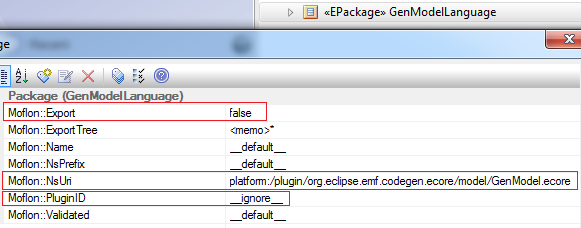
\includegraphics[width=\textwidth]{ea_genModelExportFalse}
  \caption{Update the \texttt{GenModel} export option and other tagged values}  
  \label{fig_customNS}
\end{center}
\end{figure}

\item[$\blacktriangleright$] Next we have to set the ``real'' URI of the project to be used in Eclipse so that the relevant references are exported
properly. Set the value of \texttt{Moflon::NsUri} to \texttt{platform:/\-plugin/\-org.\-eclipse.\-emf.codegen.ecore/\-model/\-GenModel.ecore}.
As the default plugin ID generation provided by eMoflon is also not valid here, set the value of \texttt{Moflon::PluginID} to \texttt{\_\_ignore\_\_} (two underscores before and after!).
The three relevant values to be set are shown in \Cref{fig_customNS}.

\item[$\blacktriangleright$] Validate and export all projects as usual to your Eclipse workspace, and update the metamodel project by pressing \texttt{F5} in
the package explorer.

\item[$\blacktriangleright$] Right-click \texttt{Ecore2GenModel} once more and navigate to ``Plug-in Tools/Open Manifest.'' The plug-in manager should have
opened in the editor with a series of tabs at the bottom.

\item[$\blacktriangleright$] Switch to the \texttt{Dependencies} tab. Press \texttt{Add} and enter \texttt{org.\-eclipse.\-emf.\-codegen.\-ecore}. This plug-in
includes both the \texttt{Ecore} and \texttt{Gen\-Mod\-el} libraries we require for successful compilation of the transformation code.

\end{enumerate}

Although we have already specified the URI of the existing project (in this example, \texttt{GenModel}) as tagged project values, we still have to 
configure a few things for code generation.

\begin{enumerate}
  
\item[$\blacktriangleright$] Expand the \texttt{Ecore2GenModel} project folder and open the \texttt{mof\-lon.\-prop\-er\-ties.\-xmi} file tree. Right-click the
properties container, and create a new \texttt{Add\-it\-ion\-al Dep\-en\-den\-cies} child. Double click the element to open its properties tab below the
editor, and as shown in \Cref{eclipse:addDepChild}, update its \texttt{Value} to:\\
\end{enumerate}

\vspace{-1cm}
{\small \ttfamily  platform:/plugin/org.eclipse.emf.codegen.ecore/model/GenModel.ecore} \\
\vspace{-0.5cm}

\begin{figure}[htbp]
\begin{centering}
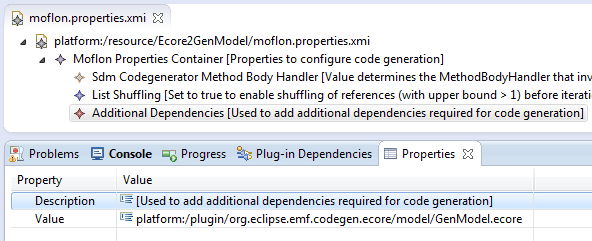
\includegraphics[width=\textwidth]{eclipse_additDepProps}
  \caption{Setting properties for code generation}  
  \label{eclipse:addDepChild}
\end{centering}
\end{figure} 

\begin{enumerate}

\item[$\blacktriangleright$] Similarly, add a second \texttt{Additional Used Gen Packages} child and set its value to: \\
\end{enumerate}

\vspace{-1cm}
{\small \ttfamily platform:\-/\-plugin/\-org.\-eclipse.\-emf.\-codegen.\-ecore/\-model/\-GenModel.\-genmodel}

\newpage
Finally, to compenstate for some cases where our naming conventions were violated, analogously add the following mapping as corrections:

\begin{enumerate}
\item[$\blacktriangleright$] Add an \emph{import mapping} child for correct generation of imports, setting the key as \texttt{genmodel} (depicted in \Cref{eclipse:impMapValues}) and value to: \\
{\small \ttfamily \hspace*{0.5cm} org.\-eclipse.\-emf.\-codegen.\-ecore.\-genmodel}

\vspace{0.5cm}

\begin{figure}[htbp]
\begin{centering}
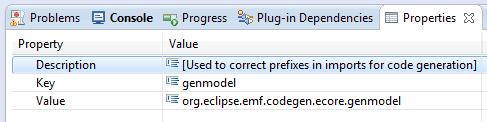
\includegraphics[width=0.9\textwidth]{eclipse_importMappingValues}
  \caption{Correcting default conventions for generating imports}  
  \label{eclipse:impMapValues}
\end{centering}
\end{figure} 

\item [$\blacktriangleright$] Finally, add a \emph{factory mapping} to ensure that \texttt{GenModelFactory} is used as the factory for creating elements in the
transformation instead of \texttt{Genmodel\-Factory}, which would be the default convention. Set its key as \texttt{genmodel}, and its value to:
{\small \ttfamily GenModelFactory}.

\item [$\blacktriangleright$] Its now time to generate code for the project.
If everything worked out and the generated code compiles, you can ensure that the transformation behaves as expected by invoking the methods and transforming an ecore file to a corresponding genmodel.

\end{enumerate}


As a final remark, note that import and factory mappings are not always necessary, \texttt{GenModel} is in this sense a particularly nasty example as it violates all our default conventions.
 